\documentclass[a4paper]{beamer}

\usepackage[english]{babel}
\usepackage[utf8]{inputenc}
\usepackage{graphicx}
\usepackage{subcaption}
\usepackage{hyperref}
\usepackage{listings}

%\usepackage{color}
\definecolor{darkgreen}{RGB}{0 100 0}

\definecolor{lightgray}{RGB}{240 240 240}
\newcommand{\code}[1]{\colorbox{lightgray}{\lstinline~#1~}}

\definecolor{light-blue}{RGB}{210,210,255}
\definecolor{light-red}{RGB}{255,210,210}
\definecolor{light-yellow}{RGB}{255, 255, 150}
\definecolor{light-grey}{RGB}{220, 220, 220}

\lstset{language=Java, tabsize=4, literate={ç}{{\c{c}}}1 {é}{{\'e}}1 {è}{{\`e}}1 {ê}{{\^e}}1 {à}{{\`a}}1 {î}{{\^i}}1 {É}{{\'E}}1 {ô}{{\^o}}1, stringstyle=\color{red}, keywordstyle=\color{blue}, identifierstyle=\color{black}, escapeinside={♠}{♣}}

\usetheme{Darmstadt}
\definecolor{clearblueifnti}{RGB}{24,116,220}
\setbeamercolor{title}{use=structure,bg=clearblueifnti,fg=white}



\makeatletter
\setbeamertemplate{title page}{
  \vbox{}
  \vfill
  \begingroup
    \centering\hspace{2cm}
    \begin{minipage}{.7\textwidth}
    \begin{beamercolorbox}[sep=8pt,center,shadow=true,rounded=true]{title}
      \usebeamerfont{title}\inserttitle\par%
      \ifx\insertsubtitle\@empty%
      \else%
        \vskip0.25em%
        {\usebeamerfont{subtitle}\usebeamercolor[fg]{subtitle}\insertsubtitle\par}%
      \fi%     
    \end{beamercolorbox}%
    \end{minipage}

    \vskip2.8em\par
    \begin{minipage}{\textwidth}
    \begin{beamercolorbox}[sep=8pt,center]{author}
      \usebeamerfont{author}\insertauthor
    \end{beamercolorbox}
    \end{minipage}

    \begin{minipage}{\textwidth}
    \begin{beamercolorbox}[sep=8pt,center]{institute}
      \usebeamerfont{institute}\insertinstitute
    \end{beamercolorbox}
    \end{minipage}

    \begin{minipage}{\textwidth}
    \begin{beamercolorbox}[sep=8pt,center]{date}
      \usebeamerfont{date}\insertdate
    \end{beamercolorbox}
    \end{minipage}
    \vskip0.5em
    {\usebeamercolor[fg]{titlegraphic}\inserttitlegraphic\par}
  \endgroup
  \vfill
}
\makeatother

\title{Docker}
\subtitle[DAP]{UE Libre}
\institute{IFNTI L3}
\author{Jean-Christophe Carré\thanks{Inspiré de la documentation Junit5 et du cours d'openclassroom sur les tests unitaires}}
\date{\today}

\setbeamertemplate{footline}
{
  \hbox{
  \begin{beamercolorbox}[wd=.3\paperwidth,ht=2.25ex,dp=1ex,center]{author in head/foot}
    \usebeamerfont{author in head/foot}\insertshortauthor
  \end{beamercolorbox}
  \begin{beamercolorbox}[wd=.6\paperwidth,ht=2.25ex,dp=1ex,center]{date in head/foot}
    \usebeamerfont{date in head/foot}\insertshortsubtitle{} : \inserttitle{} - \insertshortinstitute{} - \insertdate
  \end{beamercolorbox}
  \begin{beamercolorbox}[wd=.1\paperwidth,ht=2.25ex,dp=1ex,center]{title in head/foot}
    \usebeamerfont{title in head/foot}\insertframenumber{} / \inserttotalframenumber
  \end{beamercolorbox}}
}

\usebackgroundtemplate{
\includegraphics[width=\paperwidth,height=\paperheight]{CharteGraphiquePresentationCorps_etroit}}

\begin{document}

{
\setbeamertemplate{headline}{\vskip\headheight}
\setbeamertemplate{footline}{}
\usebackgroundtemplate{
\includegraphics[width=\paperwidth,height=\paperheight]{CharteGraphiquePresentationPageDeGarde}}
\begin{frame}[plain]
	%\vspace{5cm}
	\titlepage
\end{frame}
}

\begin{frame}{Table des matières}
	%\begin{multicols}{2}
	\tableofcontents
	%\end{multicols}
\end{frame}

{\AtBeginSection[]{
  \begin{frame}
  \vfill
  \centering
  \begin{beamercolorbox}[sep=8pt,center,shadow=true,rounded=true]{title}
    \usebeamerfont{title}\insertsection\par
  \end{beamercolorbox}
  \vfill
  \end{frame}
}

\section{Concept général}

\begin{frame}{exemple introductif}
	\begin{minipage}{0.4\textwidth}
		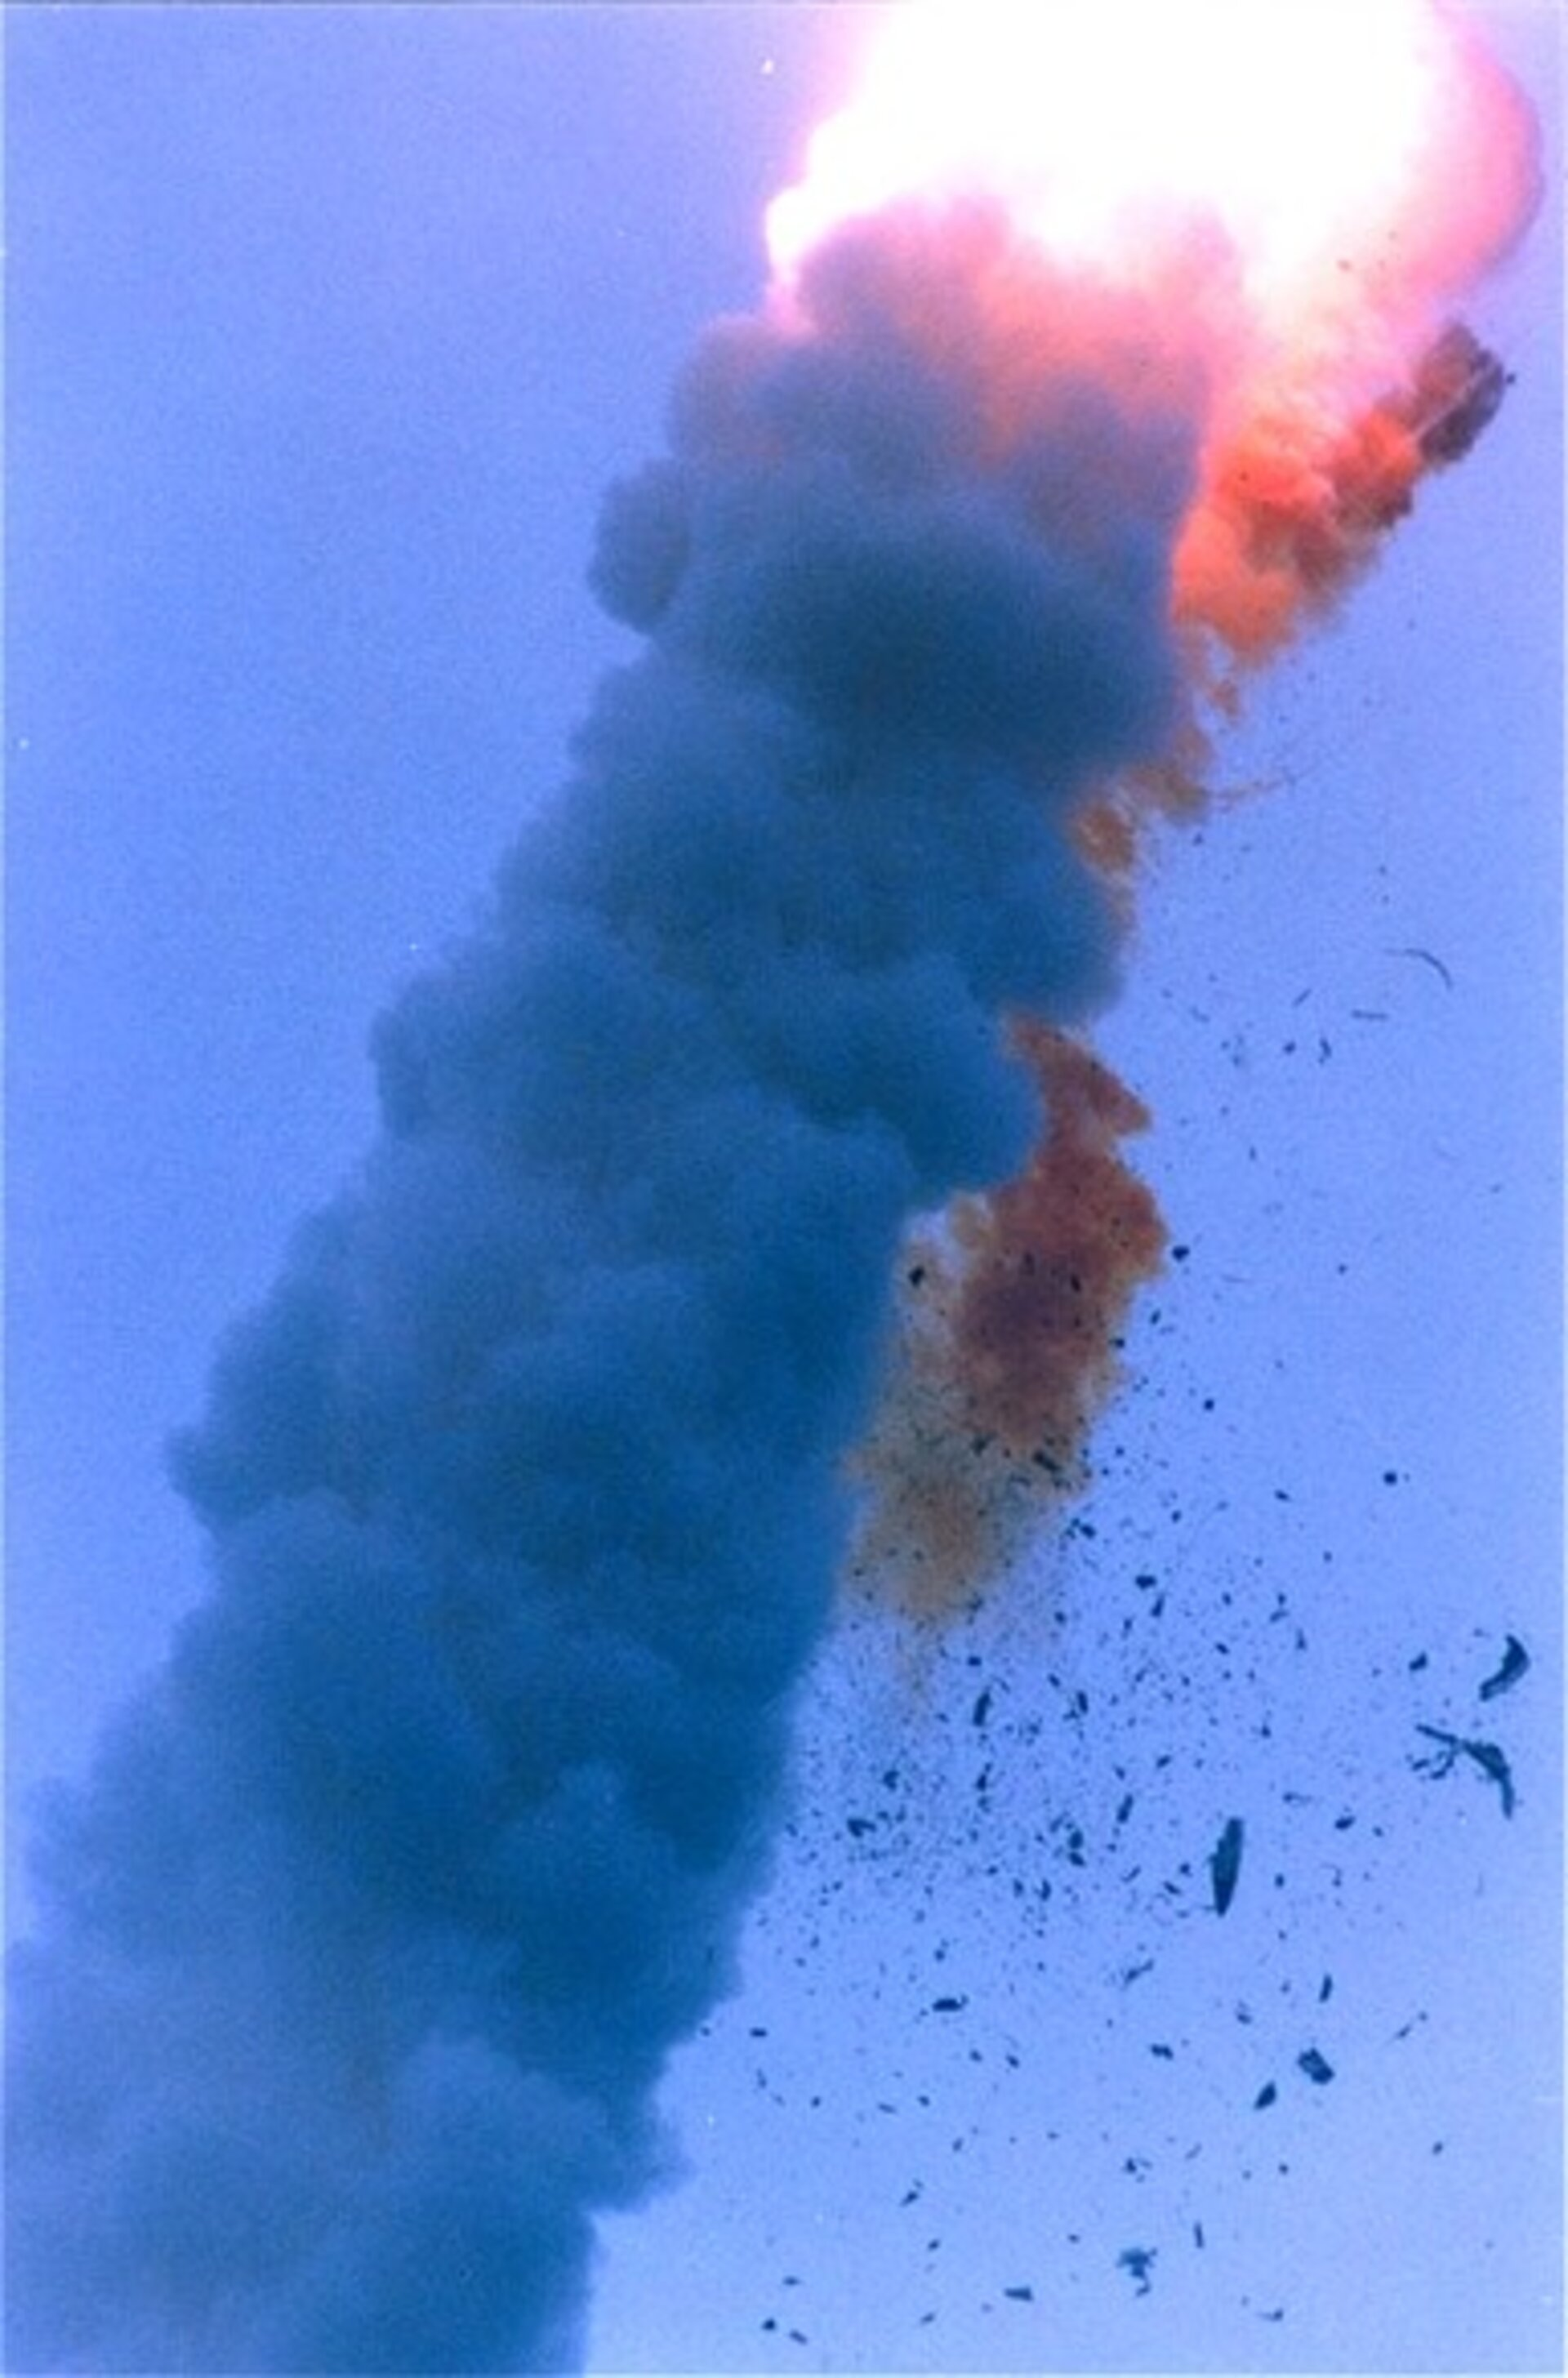
\includegraphics[height=7cm]{images/Ariane_501_explosion_pillars.jpg}
	\end{minipage}\hfill
	\begin{minipage}{0.55\textwidth}
		Ariane 501 :\\
		
		10 ans de R\&D.\\
		
		Vol inaugural, devant les caméras du monde entier.\\
		
		Tout avait été testé \tiny ou presque...
	\end{minipage}
\end{frame}

\begin{frame}{Le cycle en V}
	\noindent
	\begin{minipage}{0.45\textwidth}
		\noindent
		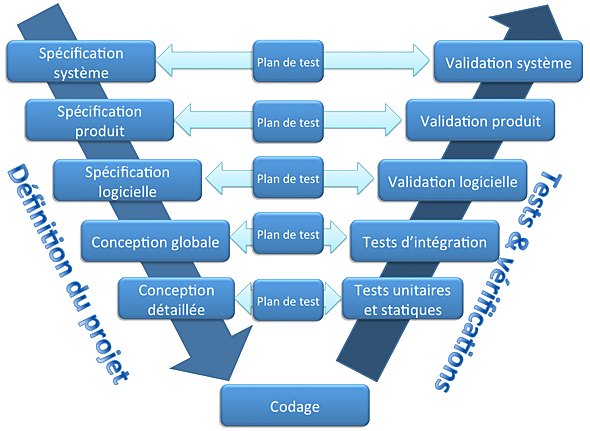
\includegraphics[width=\textwidth]{images/cycle_en_V.png}
	\end{minipage}\hfill
	\begin{minipage}{0.5\textwidth}
		Modèle d'organisation projet.\\
		Du CDC à la livraison.\\
		Détecter les erreurs au plus tôt.
	\end{minipage}
	
	\begin{block}{Test Driven Developpement (TDD)}
		Lors de la phase descendante du cycle en V, l'écriture des tests précède l'écriture du code.\\
		Les tests définissent le comportement attendu (ils sont une forme de documentation) et indiquent le travail restant.
	\end{block}

\end{frame}

\begin{frame}{La pyramide des tests : principe}
	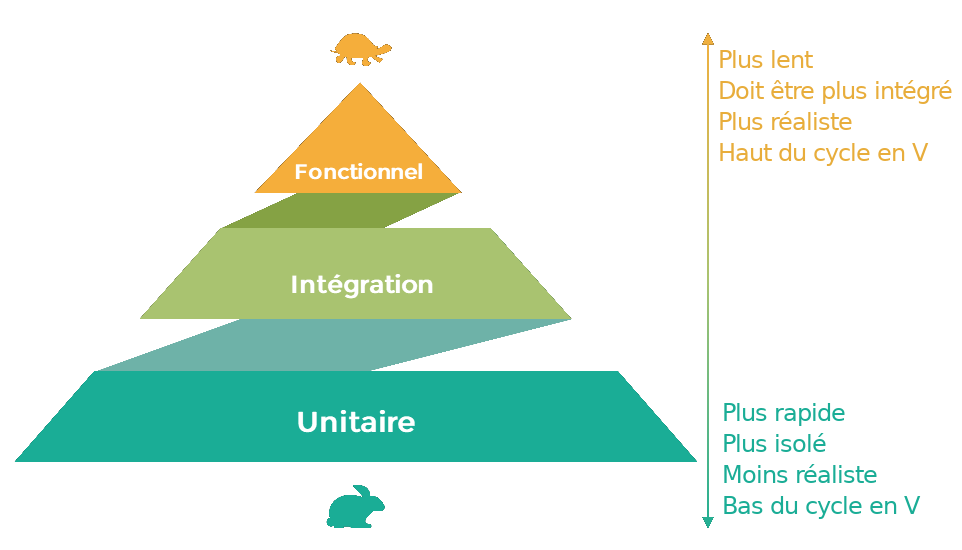
\includegraphics[width=0.95\textwidth]{images/Pyramide_des_tests2.png}
\end{frame}

\begin{frame}{La pyramide des tests : exemples}
	\begin{block}{tests unitaires}
		\begin{itemize}
			\item \small \code{lireXML("nom", "<nom>Bob</nom>")} doit renvoyer "Bob".
			\item \code{lireXML("nom", "<nom>Bob</no>")} doit lever une exception.
		\end{itemize}
	\end{block}
	\begin{block}{tests d'intégration}
		Mise en commun de différentes parties de code développées par des équipes différentes.
	\end{block}
	\begin{block}{tests fonctionnels}
		\begin{itemize}
			\item Plus d'espace de stockage sur le serveur
			\item Coupure d'alimentation de la machine
			\item Perte du réseau internet/intranet
		\end{itemize}
	\end{block}
\end{frame}
	
\begin{frame}{Manuel ou automatique}
	\begin{block}{Tests manuels}
		
		\begin{minipage}{0.44\textwidth}
			\begin{itemize}
				\item \textcolor{darkgreen}{Poussés et complexes}
				\item \textcolor{darkgreen}{Scénarios réalistes}
				\item \textcolor{darkgreen}{Aucun travail amont}
			\end{itemize}
		\end{minipage}\hfill
		\begin{minipage}{0.55\textwidth}
			\begin{itemize}
				\item \textcolor{red}{Fastidieux et répétitif}
				\item \textcolor{red}{Risque d'erreur humaine (négligence)}
			\end{itemize}
		\end{minipage}
		\vspace{0.2cm}
		\begin{center}
			Adaptés à la phase de recette du produit fini.
		\end{center}
		
	\end{block}
	
	\begin{block}{Tests automatiques}
		\begin{minipage}{0.44\textwidth}
			\begin{itemize}
				\item \textcolor{darkgreen}{Exécution immédiate}
				\item \textcolor{darkgreen}{Rigueur absolue}
			\end{itemize}
		\end{minipage}\hfill
		\begin{minipage}{0.55\textwidth}
			\begin{itemize}
				\item \textcolor{red}{Uniquement cas simples}
				\item \textcolor{red}{Nécessite du travail de codage}
				\item \textcolor{red}{Difficile d'être exhaustif}
			\end{itemize}
		\end{minipage}
		
		\vspace{0.2cm}
		\begin{center}
			Adaptés à la phase de développement itératif.
		\end{center}
		
	\end{block}
\end{frame}



\begin{frame}{Bonnes pratiques 1/2}
	
	\begin{block}{En phase de conception}
		Choix de scénarios prédéfinis et représentatifs :
		\begin{itemize}
			\item Cas nominal
			\item Tous les cas d'erreurs (NTUI).\\
		\end{itemize}
		Une modification d'une fonction peut impacter tout le reste du code. $\rightarrow$ test automatique de tout le code pour vérifier l'absence d'effets indésirables.
	\end{block}
	
	\begin{block}{En phase de production}
		Facilite la maintenance (exécution de tous les tests automatiques avant d'uploader une nouvelle version)
	\end{block}
\end{frame}

\begin{frame}{Bonnes pratiques 1/2}
\begin{block}{\textbf{F.I.R.S.T.}}
\begin{itemize}
\item \textbf{Fast} (\texttt{<} 5 ms) Pour pouvoir être souvent exécutés.\\
Utiliser l'annotation @Timeout si besoin.
\item \textbf{Isolated} Un test ne doit pas utiliser les variables ou bien les résultats d'un autre test.
\item \textbf{Repeatable} Toujours le même résultat pour un même code. (ne doit pas dépendre de la date, ou de la charge de travail de la machine)
\item \textbf{Self-validating} Ne nécessite pas de relecture pour connaître l'état validé ou non.
\item \textbf{Thourough} NTUI ! \tiny{(c.f. couverture des tests)}
\end{itemize}
\end{block}
\end{frame}

\section{TDD}
\begin{frame}{Modèle red-green-refractor}
  \begin{center}
  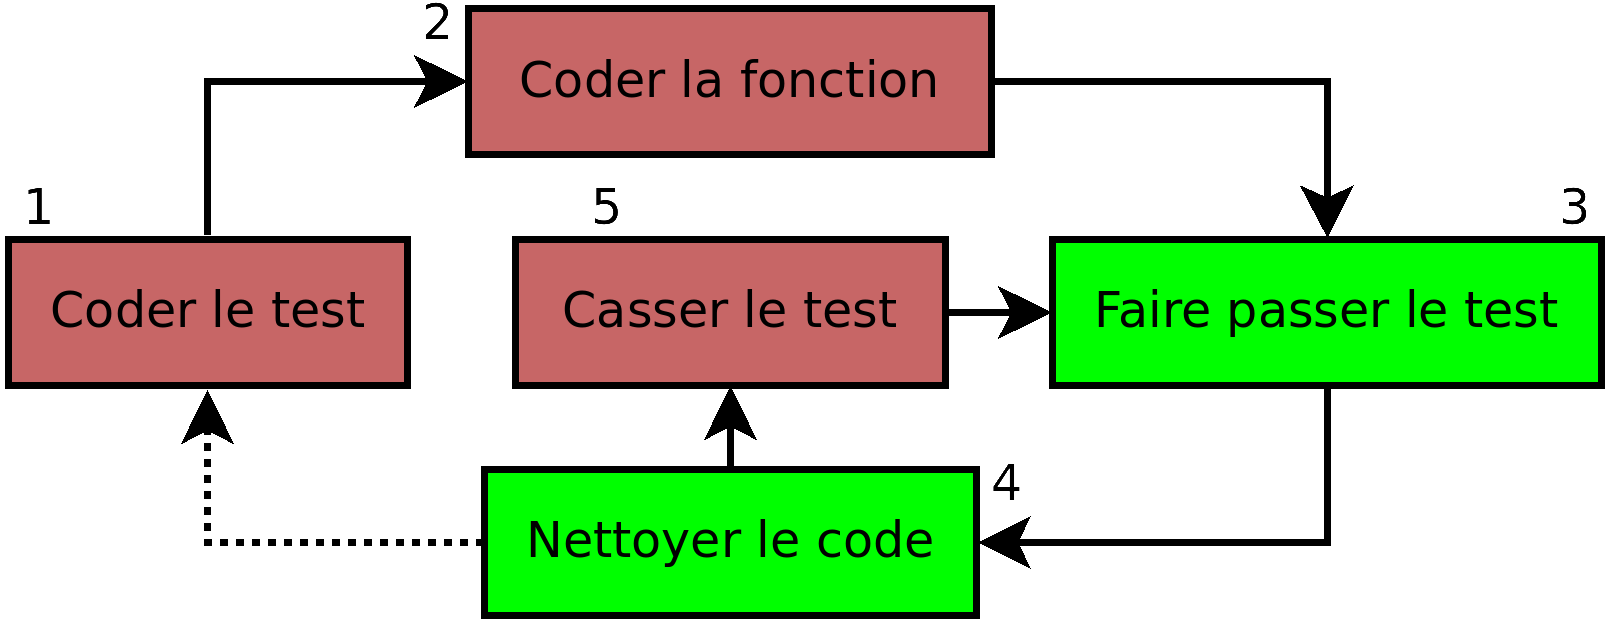
\includegraphics[width=0.8\textwidth]{images/Red-green-refractor.png}
  \end{center}
	
	\begin{block}{Tout ce qu'il faut et rien que ce qu'il faut}
		\begin{itemize}
			\item Coder le test (la fonction ne passe pas le test) $\rightarrow$ Red
			\item Coder la fonction, jusqu'à ce que le test passe $\rightarrow$ Green
			\item Nettoyer le code, en enlevant le superflu $\rightarrow$ Refract
		\end{itemize}
	\end{block}
\end{frame}


\begin{frame}{Cinématique du test}
	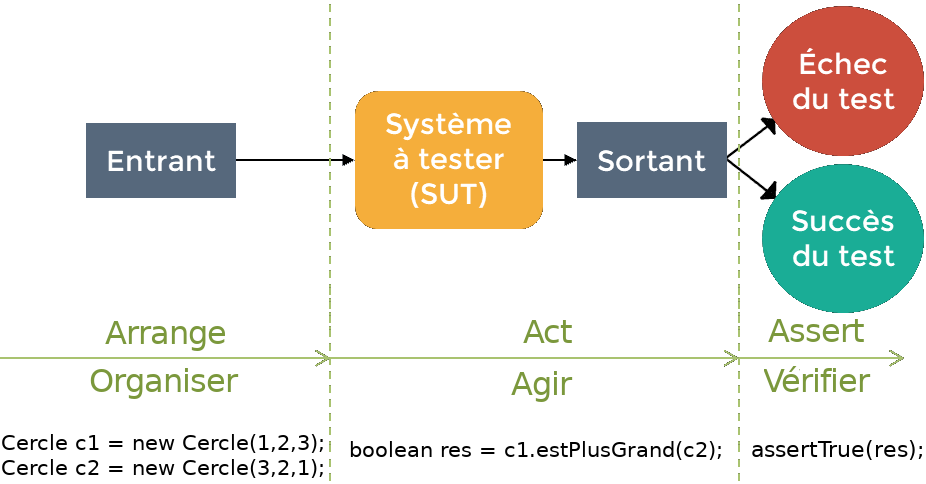
\includegraphics[width=\textwidth]{images/Cinematique_du_test_avec_exemple.png}
\end{frame}


%TODO Expliquer qu'il faut coder les tests pour qu'ils s'exécutent d'abord sur les fonctions les plus bas niveau, avant de remonter. Les tests des fonctions haut niveau ne peuvent en effet pas passer leur tests si ceux des fonctions de plus bas niveau ne passent pas. Dans la démarche TDD, c'est la même chose : en phase de développement, on commence par les fonctions de plus bas niveau.


\begin{frame}[fragile]{Assertions}
\begin{block}{But}
	Définissent les conditions de succès ou d'échec d'un test.\\
	Multiples critères possibles.\\
	Une Seule Assertion par test.\\
\end{block}
	\begin{block}{Syntaxes}
	\small
		\begin{tabular}{|p{0.28\textwidth}|p{0.62\textwidth}|}
			\hline
			Égalité de valeur & \small \texttt{assertEquals(<obtenu>, <attendu>);} \\
			\hline
			Temps d'exécution & \small \texttt{assertTimeout(ofMinutes(2), () -> \{  //tâche qui prend moins de 2 minutes \});} \\
			\hline
			Levée d'une exception & \small \texttt{assertThrows}\\
			\hline
			Non nullité & \small \texttt{assertNotNull(variable);}\\
			\hline
			Vérification booléenne & \small \texttt{assertTrue(lastName.endsWith("e"));}\\
			\hline
		\end{tabular}
	\end{block}
\end{frame}





\section{Annotations Junit}
\begin{frame}{Plus de clarté dans l'exécution}
	Permet d'afficher des messages lors de l'exécution des tests.
	\begin{itemize}
		\item \code{@Tag} regroupe tous les tests d'une classe.
		\item \code{@nested} regroupe tous les tests d'une classe interne.
		\item \code{@DisplayName} Affecte un nom à un test ou à un groupe de test.
	\end{itemize}
	\begin{center}
		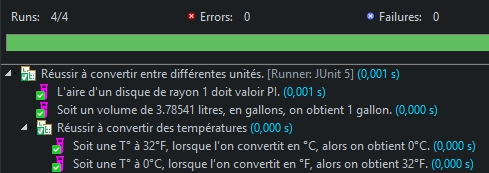
\includegraphics[width=0.9\textwidth]{images/Tests_annotes}
	\end{center}
\end{frame}

\begin{frame}{Définir la séquence d'exécution}
	\begin{itemize}
		\item \code{@BeforeAll} Partie du code qui sera exécutée une seule fois, avant tout le reste.
		\item \code{@BeforeEach} Partie du code qui sera exécutée avant chaque test.
		\item \code{@Test} Indique qu'il s'agit d'un test qui doit être exécuté (pas besoin de main)
		\item \code{@AfterEach} Partie du code qui sera exécutée après chaque test.
		\item \code{@AfterAll} Partie du code qui sera exécutée une seule fois, après tout le reste.
	\end{itemize}
\end{frame}

\begin{frame}[fragile]{Complexifier les cas de tests}
	\begin{exampleblock}{Multiples cas à tester}\scriptsize
		\begin{lstlisting}
@DisplayName("Fonction ajouter avec valeurs positives et négatives")
@ParameterizedTest(name = "{0} + {1} should equal to {2}")
@CsvSource({ "1,1,-2", "2,-3,-5", "3,-2,-7" })
public void testAdd(int arg1, int arg2, int expectResult) {
    // Arrange -- Tout est prêt !

    // Act
    int actualResult = calculatorUnderTest.add(arg1, arg2);

    // Assert
    assertEquals(expectResult, actualResult);
}
		\end{lstlisting}
	\end{exampleblock}
\end{frame}


\section{Couverture des tests}
\begin{frame}
\begin{block}{Définition}
Mesure la proportion de code qui a été exécutée lors des Tests.\\

Plusieurs mesures possibles : 
\begin{itemize}
\item Nombre de lignes
\item Nombre d'instructions
\item Nombre de branches
\item Nombre de méthodes (déconseillé)
\end{itemize}
\end{block}

\begin{block}{Exigence fixée par le contexte}
\begin{itemize}
\item Aéronautique : couverture 100\% des instructions
\item Automobile : couverture 90\%
\item Domotique : couverture 80\%
\end{itemize}

\end{block}

\end{frame}


\begin{frame}{}

\end{frame}

}
\end{document}
